\documentclass[10pt]{beamer}
\usetheme{metropolis}
\usepackage{booktabs}
\usepackage{tabularx}
\usepackage{calc}
\usepackage{tikz}

\usetikzlibrary{shapes.geometric, arrows, positioning, decorations.pathreplacing}

% Setup for faculty images
\newlength{\imageheight}
\setlength{\imageheight}{3.5cm}

% Define CSUF brand colors
\definecolor{titanblue}{HTML}{00244E}
\definecolor{mediumblue}{HTML}{0F3F8C}
\definecolor{skyblue}{HTML}{EBFBFF}
\definecolor{titanorange}{HTML}{FF7900}
\definecolor{titangray}{HTML}{F5F5F5}
\definecolor{titantext}{HTML}{222222}
\definecolor{warningred}{HTML}{D7263D} % Added missing color definition

% Customize metropolis theme colors
\setbeamercolor{normal text}{fg=titantext, bg=white}
\setbeamercolor{alerted text}{fg=titanorange}
\setbeamercolor{example text}{fg=mediumblue}

% Title page colors
\setbeamercolor{title}{fg=titanblue, bg=white}
\setbeamercolor{subtitle}{fg=mediumblue, bg=white}
\setbeamercolor{institute}{fg=titanorange, bg=white}
\setbeamercolor{date}{fg=titanblue, bg=white}

% Frame title colors
\setbeamercolor{frametitle}{fg=white, bg=titanblue}
\setbeamercolor{framesubtitle}{fg=mediumblue, bg=white}

% Block environment colors
\setbeamercolor{block title}{fg=white, bg=titanblue}
\setbeamercolor{block body}{fg=titantext, bg=skyblue!10}

% Item colors
\setbeamercolor{itemize item}{fg=titanorange}
\setbeamercolor{itemize subitem}{fg=mediumblue}
\setbeamercolor{itemize subsubitem}{fg=titanblue}

% Footer and header colors
\setbeamercolor{footer}{fg=titantext}
\setbeamercolor{header}{fg=titanblue}

% Customize fonts
\setbeamerfont{title}{size=\Large, series=\bfseries}
\setbeamerfont{frametitle}{size=\large, series=\bfseries}

% Simple title page template
\defbeamertemplate*{title page}{customized}[1][]
{
\vspace{1cm}
 {\usebeamerfont{title}\usebeamercolor[fg]{title}\inserttitle\par}
\vspace{0.5cm}
 {\usebeamerfont{subtitle}\usebeamercolor[fg]{subtitle}\insertsubtitle\par}
\vspace{0.5cm}
 {\usebeamerfont{date}\usebeamercolor[fg]{date}\insertdate\par}
\vfill
 {\insertinstitute\par}
}

% Add progress bar
\makeatletter
\setbeamertemplate{headline}{%
\begin{beamercolorbox}[wd=\paperwidth,ht=0.4cm,dp=0cm]{titanblue}%
\begin{tikzpicture}
\pgfmathsetmacro{\progress}{\insertframenumber/\inserttotalframenumber}
\fill[titanorange] (0,0) rectangle (\progress*\paperwidth,0.4cm);
\end{tikzpicture}%
\end{beamercolorbox}%
}
\makeatother

\begin{document}

\title{Understanding Politics and Public Policy}
\subtitle{Foundations and Core Concepts \\ POSC 315: Introduction to Public Policy \\ Lecture 8-3: Decision Making (Part 3 of 3)}
\date{David P. Adams, Ph.D.}
\institute{California State University, Fullerton}

\maketitle

\begin{frame}{Decision-Making Models Overview}
\begin{itemize}
  \item \textbf{Rational Choice:} Idealized model based on full information and optimization.
  \item \textbf{Bounded Rationality:} Limited information and satisficing behavior.
  \item \textbf{Incrementalism:} Policy change through small, conservative steps.
  \item \textbf{Groupthink:} When group harmony overrides critical thinking.
  \item \textbf{Garbage Can Model:} Organized anarchy; decisions emerge from timing.
\end{itemize}
\end{frame}

\begin{frame}{Groupthink: Key Symptoms}
\begin{block}{Definition}
Prioritizing group cohesion and unanimity over critical analysis.
\end{block}
\vspace{0.5cm}
\textbf{Common Symptoms:}
\begin{itemize}
  \item Illusion of invulnerability
  \item Collective rationalization
  \item Suppression of dissent
  \item Self-censorship
\end{itemize}
\end{frame}

\begin{frame}{Garbage Can Model of Decision-Making}
\begin{block}{Core Idea}
Problems, solutions, participants, and choice opportunities float independently and only occasionally align.
\end{block}
\begin{itemize}
  \item Developed by Cohen, March, and Olsen (1972)
  \item Reflects high-uncertainty, loosely coupled organizations
\end{itemize}
\end{frame}

\begin{frame}{Four Streams in the Garbage Can Model}
\begin{itemize}
  \item \textbf{Choices} looking for problems
  \item \textbf{Issues} looking for decision venues
  \item \textbf{Solutions} looking for problems
  \item \textbf{Participants} looking for something to do
\end{itemize}
\textbf{When these converge by chance:} a decision is made.
\end{frame}

\begin{frame}{Garbage Can Model: Streams Visualization}
\centering
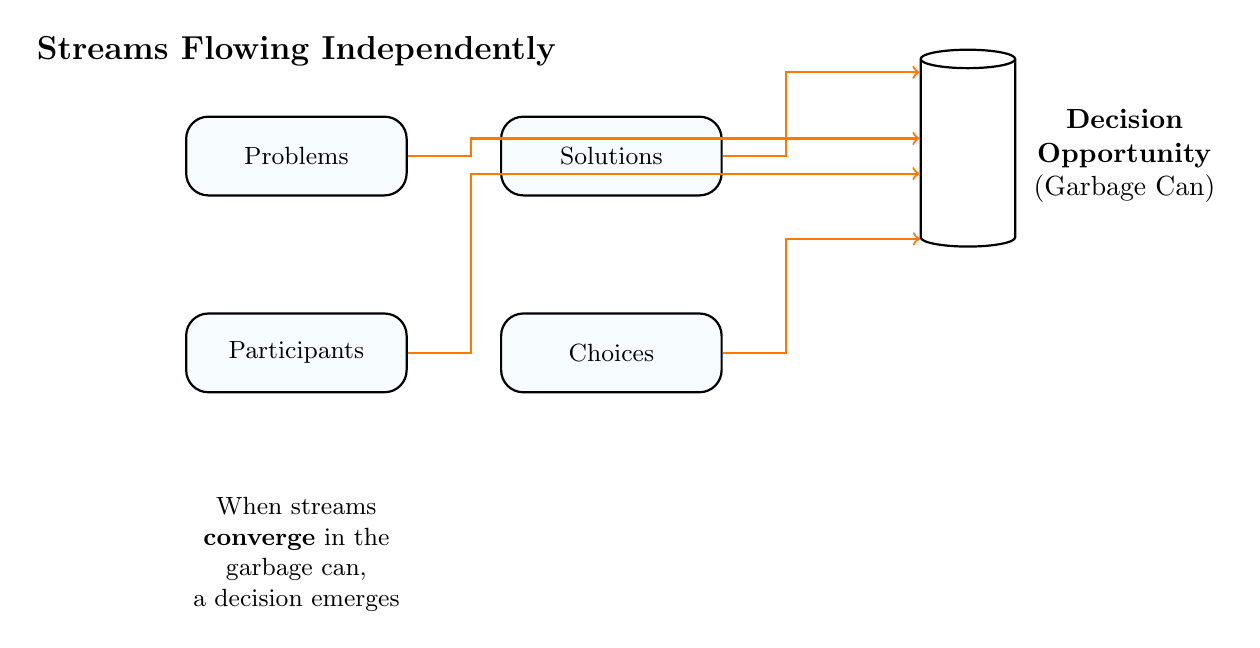
\begin{tikzpicture}[
    stream/.style={draw, thick, rounded corners=8pt, minimum width=2.8cm, minimum height=1cm, font=\small, fill=skyblue!40},
    arrow/.style={->, thick, titanorange},
    every node/.style={align=center}
  ]
  % Shift everything further left to avoid cutoff
  \begin{scope}[xshift=-3.2cm]
    % Streams
    \node[stream] (problems) at (0,2.5) {Problems};
    \node[stream] (solutions) at (4,2.5) {Solutions};
    \node[stream] (participants) at (0,0) {Participants};
    \node[stream] (choices) at (4,0) {Choices};

    % Garbage can (decision opportunity)
    \node[draw, thick, cylinder, shape border rotate=90, minimum height=2.5cm, minimum width=1.2cm, fill=white, right=2.5cm of solutions, label=right:{\parbox{2.5cm}{\centering \textbf{Decision\\ Opportunity}\\ (Garbage Can)}}] (can) {};

    % Arrows from streams to can
    \draw[arrow] (problems.east) -- ++(0.8,0) |- (can.160);
    \draw[arrow] (solutions.east) -- ++(0.8,0) |- (can.120);
    \draw[arrow] (participants.east) -- ++(0.8,0) |- (can.200);
    \draw[arrow] (choices.east) -- ++(0.8,0) |- (can.240);

    % Labels
    \node[above=0.5cm of problems, font=\bfseries\large, align=center] {Streams Flowing Independently};
    \node[below=1.2cm of participants, align=center, font=\small] {When streams\\\textbf{converge} in the\\garbage can,\\a decision emerges};
  \end{scope}
\end{tikzpicture}
\end{frame}

\begin{frame}{Comparison Table: Decision-Making Models}
\begin{tabularx}{\textwidth}{l X X X}
\toprule
\textbf{Model} & \textbf{Information} & \textbf{Process} & \textbf{Outcome} \\
\midrule
Rational Choice & Complete & Optimization & Best solution \\
Bounded Rationality & Limited & Satisficing & Good enough \\
Incrementalism & Limited & Small steps & Gradual change \\
Groupthink & Filtered & Conformity & Poor decisions \\
Garbage Can & Random & Stream convergence & Unpredictable \\
\bottomrule
\end{tabularx}
\end{frame}

\begin{frame}{Decision-Making Toolkit}
\begin{itemize}
  \item \textbf{Rational Analysis} -- When info is good
  \item \textbf{Satisficing} -- When time is short
  \item \textbf{Incrementalism} -- When risk is high
  \item \textbf{Groupthink Prevention} -- Build in dissent
  \item \textbf{Opportunity Recognition} -- Be ready when streams align
\end{itemize}
\end{frame}

\begin{frame}{Final Thought}
\begin{quote}
\textbf{``The best decision-makers aren't those who follow one model perfectly, but those who know which model to use when.''}
\end{quote}
\end{frame}

\end{document}
